\section{Motivation}
\label{motivation}

%The amount of biological data is increasing exponentially, both in terms of data available in biomedical databases as in the amount of published literature.
In recent years, there has been an exponential increase in the research of biological domain, much due to the extensive use of high-throughput technologies such as yeast-two hybrid-based methods, DNA expression arrays and mass spectrometry.
These methods have been producing large and heterogeneous collections of data, including proteomic and genomic sequence data, expression profiles, and protein structure coordinates that represent an important fraction of existing biological information \citep{buckingham2004}.
High-throughput technologies generate massive amounts of data that in turn require efficient information retrieval before any analysis is attempted.
Since the 19th century, natural language is the main vehicle through which humans transmit and exchange the facts discovered in biological research, by means of scientific publications, patents, or reports \citep{searls2001}.
The most comprehensive repository for such articles is the MEDLINE database \citep{greenhalgh1997}.
MEDLINE is a bibliographic database of life sciences and biomedical information that currently contains over 19 million records that can be accessed through PubMed.
Figure \ref{medline} shows the exploding number of articles available from MEDLINE since its creation in 1965, showing the exponential growth of published biomedical documents.

\begin{figure} %figure1
\centerline{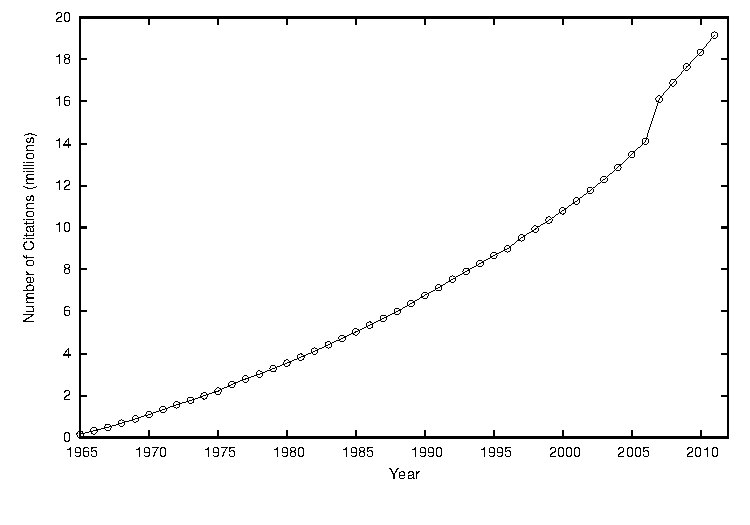
\includegraphics[width=15cm]{SupportFiles/plots/pubmedgrowth.pdf}}
	\caption[Medline growth.]{Number of citations present in MEDLINE since its beginning in 1950. Data from official statistics available at \url{www.nlm.nih.gov/bsd/index\_stats\_comp.html}.}
\label{medline}
\end{figure}

%Technological advances and professional competition have contributed to the large volume of scientific articles, making it impossible for researchers to keep up with the literature.


\section{Objectives}

% set the hypothesis here, use it where needed with \hypothesis
\newcommand{\hypothesis}{
\begin{description}
	\item[Hypothesis:] The results achieved by current chemical entity identification systems can be improved by exploiting a Machine Learning approach and Semantic Similarity techniques using dictionaries as domain knowledge. 
\end{description}
}

\hypothesis


\section{Contributions}


Thus, the following specific contributions can be enumerated as follows:
\begin{description}
	\item[Contribuition1:] 
\end{description}


\section{Overview}

The overview of this document is as follows.


